\documentclass[11pt]{article}
\usepackage{amsmath,amssymb,amsthm}
\usepackage{cite}
\usepackage{tikz}
\usetikzlibrary{shapes}

\DeclareMathOperator*{\E}{\mathbb{E}}
\let\Pr\relax
\DeclareMathOperator*{\Pr}{\mathbb{P}}
\DeclareMathOperator*{\Oh}{\mathcal{O}}

\newcommand{\eps}{\varepsilon}
\newcommand{\inprod}[1]{\left\langle #1 \right\rangle}
\newcommand{\R}{\mathbb{R}}

\newcommand{\handout}[5]{
  \noindent
  \begin{center}
  \framebox{
    \vbox{
      \hbox to 5.78in { {\bf CS 224: Advanced Algorithms } \hfill #2 }
      \vspace{4mm}
      \hbox to 5.78in { {\Large \hfill #5  \hfill} }
      \vspace{2mm}
      \hbox to 5.78in { {\em #3 \hfill #4} }
    }
  }
  \end{center}
  \vspace*{4mm}
}

\newcommand{\lecture}[4]{\handout{#1}{#2}{#3}{Scribe: #4}{Lecture #1}}

\newtheorem{theorem}{Theorem}
\newtheorem{corollary}[theorem]{Corollary}
\newtheorem{lemma}[theorem]{Lemma}
\newtheorem{observation}[theorem]{Observation}
\newtheorem{proposition}[theorem]{Proposition}
\newtheorem{definition}[theorem]{Definition}
\newtheorem{claim}[theorem]{Claim}
\newtheorem{fact}[theorem]{Fact}
\newtheorem{assumption}[theorem]{Assumption}

% 1-inch margins, from fullpage.sty by H.Partl, Version 2, Dec. 15, 1988.
\topmargin 0pt
\advance \topmargin by -\headheight
\advance \topmargin by -\headsep
\textheight 8.9in
\oddsidemargin 0pt
\evensidemargin \oddsidemargin
\marginparwidth 0.5in
\textwidth 6.5in

\parindent 0in
\parskip 1.5ex
\usepackage{todonotes}

\begin{document}

\lecture{7 --- September 23, 2014}{Fall 2014}{Prof.\ Jelani Nelson}{Jaroslaw Blasiok}

\section{Overview}

In this lecture we cover Splay Trees, first introduced and analyzed by Sleator and Tarjan in \cite{DBLP:journals/jacm/SleatorT85}. Splay tree is a comparison based data structure (in particular --- Binary Search Tree), which --- in contrast to BST data structures such as AVL tree and Red-Black tree --- does not maintain a property of being balanced in any way. Thus, in the worst case, complexity of a single operation could be linear in the size of structure. Nevertheless, thanks to its {\it self-adjusting} it has a bunch of interesting properties in terms of amortized guarantees --- in particular, the amortized cost of a single operation is at most $\Oh(\log n)$, matching worst-case bounds obtained by balanced binary tree. Moreover, often when sequence of inputs is structured in additional way (for example: the sequence is in some sense {\it local}, or frequencies of accessing items are far from uniform), the upper bounds for a sequence of operations are significantly better then those given by balanced binary search trees. More about this in Section~\ref{Properties}.

It should be noted, that this data structure has great practical application. In particular, in 1999 Sleator and Tarjan were granted a {\it Paris Kanellakis Theory and Practice Award}, which is given to honor {\it specific theoretical accomplishments that have had a significant and demonstrable effect on the practice of computing} in 1999, with a note: {\it For creating the Splay-Tree Data Structure [\dots ,] one of the most widely used data structures invented in the last 20 years}.

\section{Problem formulation and model}
\subsection{Problem formulation}
Our data structure will support following operations:
\begin{itemize}
	\item {\bf \underline{Insert}$(k, v)$} --- inserts new item with key $k$ and value $v$.
	\item {\bf \underline{Find}$(k)$} --- finds value associated with item $v$.
	\item {\bf \underline{Delete}$(k)$} --- deletes from data structure value associated with key $k$
\end{itemize}

Those are exactly operations that are defining {\it dictionary problem} in data structures --- one which is traditionally approached by hash tables. Here we insist that the data structure we provide is comparison based (the only operation available on keys, apart from copying and storing them, is comparison). Moreover, the data structure we provide, will actually fit in much more strict model: namely BST model. Such data structures usually can be {\it enriched} to support more complex operations such as various forms of range queries and range updates, or predecessor problem.
\subsection{BST model}
At the beginning of each operation our program is allowed to have only a single pointer to the root of a tree --- which is required to be a {\it Binary Search Tree}, i.e. every node has at most two children and exactly a single key $k$, all the nodes in left subtree should have keys smaller then $k$, all the nodes in right subtree should have keys larger than $k$. The operations we are allowed to use, is to follow a pointer to any child or a parent, or do a rotation. Rotation of node $x$, with a parent $y$ basically makes $x$ a parent of $y$ preserving a BST property --- there is only one way of doing it locally, and it is presented on Figure~\ref{rotate}.
\begin{figure}
\begin{center}
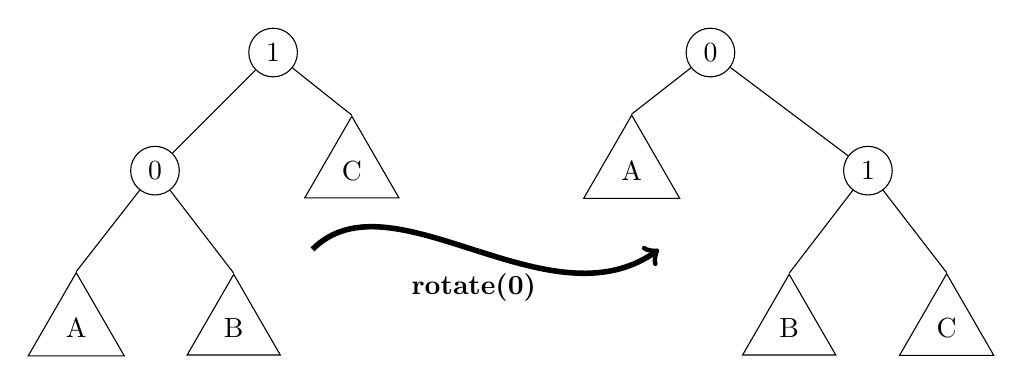
\begin{tikzpicture}[nodes=draw,shape=circle]
\tikzstyle{subtree}=[regular polygon,regular polygon sides=3]
\node[subtree] (A) at (0,0) {A};
\node[subtree] (B) at (2,0) {B};
\node[subtree] (C) at (3.5,2) {C};
\node (0) at (1,2) {0};
\node (1) at (2.5,3.5) {1};

\draw (0) -- (1) -- (C.north);
\draw (A.north) -- (0) -- (B.north);

\draw[->,line width=2] (3,1) .. controls (4,2) and (6,0) .. (7.4,1) node[midway,draw=none,below=-0.5] {\bf rotate(0)};
\begin{scope}[xshift=30]
\node[subtree] (A') at (6,2) {A};
\node[subtree] (B') at (8,0) {B};
\node[subtree] (C') at (10,0) {C};
\node (0') at (7,3.5) {0};
\node (1') at (9,2) {1};
\draw (0') -- (1') -- (C'.north);
\draw (A'.north) -- (0');
\draw (1') -- (B'.north);
\end{scope}
\end{tikzpicture}
\end{center}
\caption{\label{rotate}Single rotate operation on binary search tree.}
\end{figure}
\section{Splay trees}
The most important internal operation in the Splay tree data structure is ${\bf \underline{Splay}(x)}$. This operation in a sequence of rotations lift the element $x$ to the root of the tree, in such a way, so that it significantly improves a structure of the tree if the path to $x$ were long in the first place. Before we discuss how this operation is realized, and analyze its complexity, lets see how to define all other operations of splay tree in terms of splay operation. For a time being we only need to know that in effect of a splay operation on a node $x$, node $x$ is a root of BST containing the same elements as the one before splay operation.
\begin{itemize}
	\item {\bf \underline{Insert}$(k, v)$} --- follows child pointers as usually in BST, to find appropriate place to insert key $k$, creates new node there, then splay on this node.
	\item {\bf \underline{Find}$(k)$} --- finds a value in BST, then splay on the node containing it.
	\item {\bf \underline{Delete}$(k)$} --- finds a node with key $k$, splay it. One obtains two BSTs $L$ and $R$ out of the left and right subtree of $k$. Splay the minimum element in the $R$, then set $L$ as a left child of the root of $R$. Note that after splaying minimum element in $R$ root does not have a left child.
\end{itemize}

It is easy to see, that we can charge the cost of finding an element in BST (thus: descending a path to it, based on results of comparisons), to subsequent splay operations. Therefore it is enough to understand the amortized complexity of all splay operations in the data structure. This analysis will be presented in Section~\ref{splay}. Before we do it, lets review some interesting properties of splay tree in terms of amortized complexity.
\section{Properties}
\label{Properties}

We will state a set of properties of a data structure desirable by us. Some of them are proven to hold for splay trees, some are conjectured. For a time being lets assume that we are interested in total complexity of a sequence which consists only of find() operations. We can assume also, that keys are just natural numbers $\{1, \ldots, n\}$, as only the ordering of keys matters for a comparison based data structure.
\begin{itemize}
	\item {\bf Static Optimality} --- proven for Splay Trees in \cite{DBLP:journals/jacm/SleatorT85}. \\
		Given a sequence of find operations, for any fixed binary tree $T$ we have:
		\begin{equation*}
			\text{time to perform all operations with splay tree} = \Oh(\text{time to perform all operations with T})
		\end{equation*}

		Note, that in particular it means that average cost of an operation is upper bounded by $\Oh(\log n)$, thus splay trees are on average no worse than balanced tree. Moreover, if the frequencies of items are far from equal (i.e. probability distribution on the items is far from uniform), they perform significantly better. Thus, they can perform only by a constant factor worse then optimal BST constructed for this set of frequencies, even though when using splay trees one does not have to know in advance what the set of frequencies is.
	\item {\bf Working Set} --- proven for Splay Trees in \cite{DBLP:journals/jacm/SleatorT85}. \\
		Let $t_j$ to be the number of items accessed since the last time we saw the $j-th$ item in a sequence of operations. Splay trees achieve:
		\begin{equation*}
			\Oh(m + n \log n + \sum_{i=0}^m \log(t_j)
		\end{equation*}

		This should be interpreted as follows: splay trees perform significantly better than balanced BSTs  when the sequence of operations is time local. For example queries a small set of items over and over again, then switches to another small set of items and focus on it for a longer time. This kind of local query pattern is actually sometimes reasonable assumption in real life applications.
	\item {\bf Static finger property} --- proven for Splay Trees in \cite{DBLP:journals/jacm/SleatorT85} \\
		Let $f$ be any fixed item. Then amortized cost of find(i) in splay tree is:
		\begin{equation*}
			\Oh(\log(|f - i| + 1) + 1)
		\end{equation*}

		A reasonable interpretation of property is following: splay trees performs significantly better than balanced BST if a sequence of queries is very space local, for example there is a large number of queries near a given item $i_1$, succeeded by a large number of queries near a given item $i_2$, and so on. Again this locality is reasonable in real life applications.
	\item {\bf Dynamic finger property} --- proven for Splay Trees by Cole, Mishra, Schmidt, Siegel in \cite{DBLP:journals/siamcomp/ColeMSS00}\cite{DBLP:journals/siamcomp/Cole00} \\
		If the access sequence is $\sigma_1, \sigma_2, \ldots, \sigma_m$, then the amortized cost of the $i$-th operation is:
		\begin{equation*}
			\Oh(\log(|\sigma_i - \sigma_{i+1}| + 1) + 1)
		\end{equation*}

		This again guarantees good behaviour of the splay tree with respect to space local query sequences: in particular, if elements are accessed in consecutive order, we will expect average cost of an operation to be constant.
	\item {\bf Unified Property} --- Splay trees are not known yet to have this property. This property was introduced by Iacomo in \cite{DBLP:conf/soda/Iacono01a}. \\
		If the access sequence is $\sigma_1, \sigma_2, \ldots, \sigma_m$, then the amortized cost of the $i$-th operation is:
		\begin{equation}
			\Oh(\mathrm{min}_{i < j} \log(|\sigma_i - \sigma_j| + j-i + 1) + 1) \label{ub}
		\end{equation}
		This property unifies both dynamic finger property and working set property, and it is conjectured in the same paper by Iacomo that splay trees indeed do have this property. Iacomo in \cite{DBLP:conf/soda/Iacono01a} gives other comparison based data structure, which does have the Unified Property, unfortunately it is not a BST data structure, and it is significantly more complicated than splay trees (requires 21 pointers per node).

		Later Derryberry and Sleator~\cite{DBLP:conf/wads/DerryberryS09} provided a BST data structure obtaining time cost for a sequence of form
		\begin{equation*}
			\Oh(m\log\log n + \mathrm{UB}(\sigma)
		\end{equation*}
		where UB($\sigma$) is unified bound for the sequence, i.e. sum of costs as in equation~(\ref{ub}) over all $j$.
	\item {\bf Dynamic Optimality Property} --- Splay Trees are still not known to have this property. They were conjectured to have it in the original paper \cite{DBLP:journals/jacm/SleatorT85} \\
		Let OPT($\sigma$) be the optimal cost of servicing access sequence $\sigma$ in the BST model (i.e. if one knows the entire sequence in the advance). Then dynamic optimality property is that total time of serving a sequence $\sigma$ is upper bounded by $c\, \mathrm{OPT}(\sigma)$ for some universal constant $c$.

		Splay trees are conjectured to have this property, and it is the most important unsolved conjecture about splay trees at the time: it remains unsolved for almost 30 years.

		Note that, trivially a cost of serving sequence $\sigma$ with splay trees is upper bounded by $\Oh(\log n \, \mathrm{OPT}(\sigma))$. Demaine, Harmon, Iacono and Patrascu in~\cite{DBLP:conf/focs/DemaineHIP04} gave a data structure which achieves $\mathrm{cost}(\sigma) \leq \Oh(\mathrm{OPT}(\sigma)\, \log \log n)$.
\end{itemize}
\section{Splay operation}
\label{splay}
\subsection{Operation}
In this section we will tell the details of realizing splay operation. We would like to remind at this point, that as a result of a splay operation on a given node, this node should be lifted up to a root of the tree. The naïve way of doing this would be to perform a sequence of rotate operations on a given node, until the node becomes a root of the tree. As we see on Figure~\ref{gorot} if the tree was in fact a long list (i.e. of height $n$), such a sequence of rotate operations would result in a tree again of height $n$. Thus, if one performed a sequence of $n$ splay operations on the lowest leaf of the tree, the total time of such a sequence would be of order $\Omega(n^2)$.
\begin{figure}
\begin{center}
\usetikzlibrary{shapes}
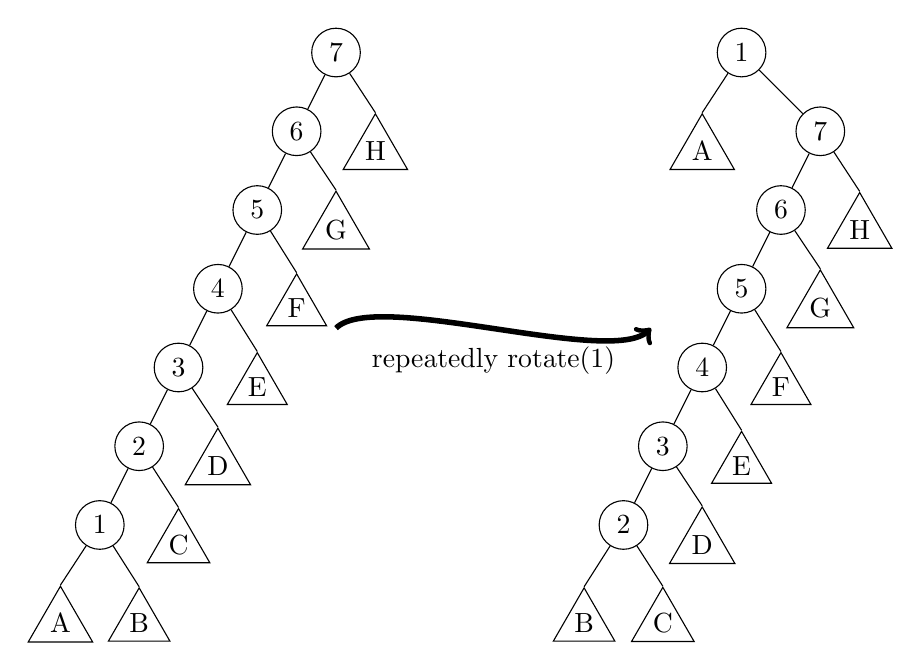
\begin{tikzpicture}[nodes=draw,shape=circle,scale=0.5]
\tikzstyle{subtree}=[regular polygon,regular polygon sides=3,inner sep=1]
\begin{scope}
\foreach \x in {1,2,...,7}{
\node(\x) at (\x, 2*\x) {\x};
};
\foreach \x/\y in {1/B,2/C,3/D,4/E,5/F,6/G,7/H}{
\node[subtree] (\y) at (\x+1, 2*\x-2.5) {\y};
\draw (\x) -- (\y.north);
};
\foreach \x/\y in {1/2,2/3,3/4,4/5,5/6,6/7}{
\draw (\x) -- (\y);
}
\node[subtree] (A) at (0,-0.5) {A};
\draw (A.north) -- (1);
\end{scope}
\draw[->,line width=2] (7,7) .. controls (8,8) and (14,6) .. (15,7) node[below=-1.3,midway,draw=none] {repeatedly rotate(1)};
\begin{scope}[xshift=350]
\foreach \x in {2,...,7}{
\node(\x) at (\x, 2*\x-2) {\x};
};
\node (1) at (5,14) {1};
\foreach \x/\y in {2/C,3/D,4/E,5/F,6/G,7/H}{
\node[subtree] (\y) at (\x+1, 2*\x-4.5) {\y};
\draw (\x) -- (\y.north);
};
\foreach \x/\y in {1/7,2/3,3/4,4/5,5/6,6/7}{
\draw (\x) -- (\y);
}

\node[subtree] (B) at (1,-0.5) {B};
\node[subtree] (A) at (4,11.5) {A};
\draw (B.north) -- (2);
\draw (A.north) -- (1);
\end{scope}
\end{tikzpicture}
\end{center}
\caption{\label{gorot}Repeatedly rotating element in a list-like tree}
\end{figure}

We will do something slightly more complicated: let us consider node $x$, its parent $y$, and $z$ --- parent of node $y$.
There are three cases:
\begin{figure}
\begin{center}
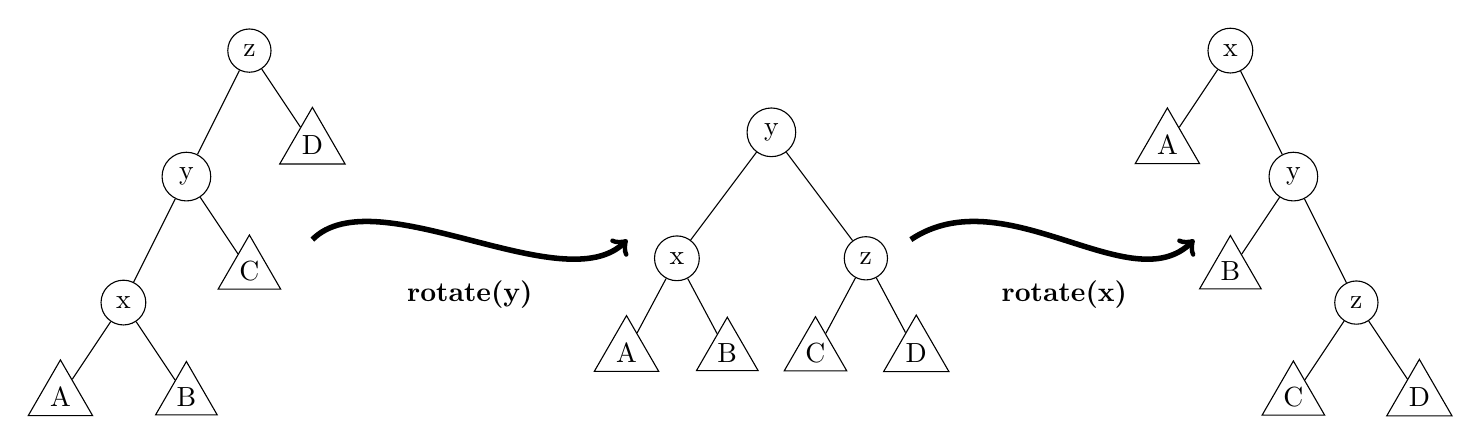
\begin{tikzpicture}[nodes=draw,shape=circle,scale=0.8]
\tikzstyle{subtree}=[regular polygon,regular polygon sides=3,inner sep=1]
\begin{scope}
\node (x) at (0,0) {x};
\node (y) at (1,2) {y};
\node (z) at (2,4) {z};
\node[subtree] (A) at (-1, -1.5) {A};
\node[subtree] (B) at (1, -1.5) {B};
\node[subtree] (C) at (2, 0.5) {C};
\node[subtree] (D) at (3, 2.5) {D};
\draw (x)--(y)--(z);
\draw (A) -- (x) -- (B);
\draw (C) -- (y);
\draw (D) -- (z);
\end{scope}
\draw[->,line width=2] (3,1) .. controls (4,2) and (7,0) .. (8,1) node[below=-0.3,midway,draw=none] {\bf rotate(y)};
\draw[->,line width=2] (12.5,1) .. controls (14,2) and (16,0) .. (17,1) node[below=-0.3,midway,draw=none] {\bf rotate(x)};
\begin{scope}[xshift=250,yshift=20]
\node (x) at (0,0) {x};
\node (y) at (1.5,2) {y};
\node (z) at (3,0) {z};
\node[subtree] (A) at (-0.8, -1.5) {A};
\node[subtree] (B) at (0.8, -1.5) {B};
\node[subtree] (C) at (2.2, -1.5) {C};
\node[subtree] (D) at (3.8, -1.5) {D};
\draw (x)--(y)--(z);
\draw (A) -- (x) -- (B);
\draw (D) -- (z) -- (C);
\end{scope}
\begin{scope}[xshift=500]
\node (x) at (0,4) {x};
\node (y) at (1,2) {y};
\node (z) at (2,0) {z};
\node[subtree] (A) at (-1, 2.5) {A};
\node[subtree] (B) at (0, 0.5) {B};
\node[subtree] (C) at (1, -1.5) {C};
\node[subtree] (D) at (3, -1.5) {D};
\draw (x)--(y)--(z);
\draw (A) -- (x);
\draw (B) -- (y);
\draw (D) -- (z) -- (C);
\end{scope}
\end{tikzpicture}
\end{center}
\caption{\label{zig-zig}Zig-zig step in splay operation (Case 2)}
\end{figure}
\begin{itemize}
\item {\bf Case 1 (zig):} Parent of $x$ is a root of the tree --- we just do rotate($x$).
\item {\bf Case 2 (zig-zig):} $x$ is left child of $y$ and $y$ is left child of $z$ or symmetric: in this case we do rotate($y$) and rotate($x$) as on Figure~\ref{zig-zig}
\item {\bf Case 3 (zig-zag):} $x$ is left child of $y$ and $y$ is right child of $z$, or symmetric: in this case we do rotate($x$) followed by rotate($x$).
\end{itemize}

\begin{figure}
\begin{center}
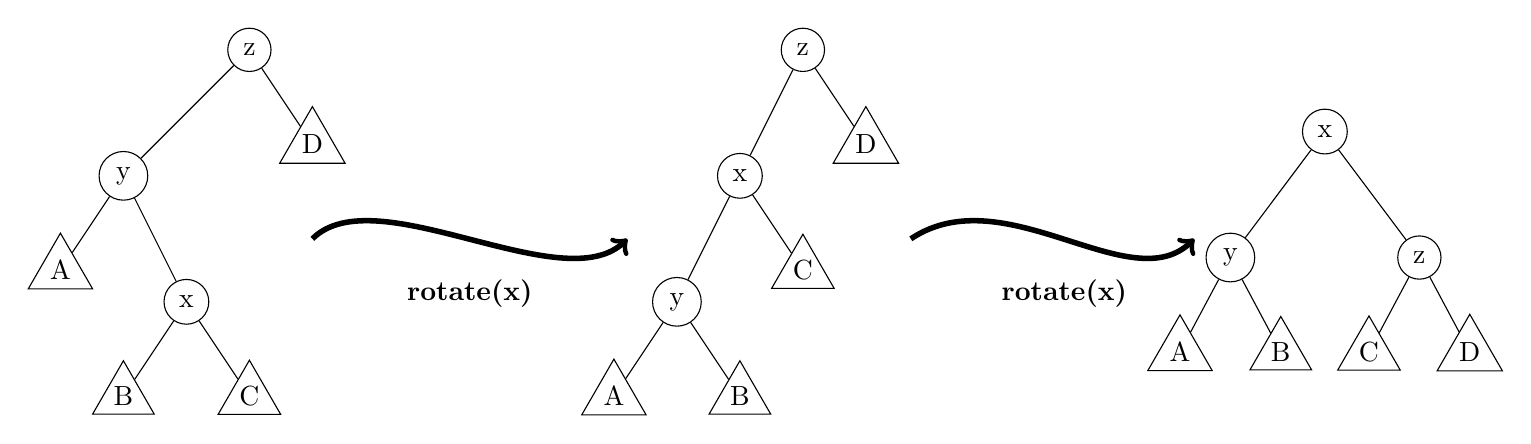
\begin{tikzpicture}[nodes=draw,shape=circle,scale=0.8]
\tikzstyle{subtree}=[regular polygon,regular polygon sides=3,inner sep=1]
\begin{scope}
\node (x) at (1,0) {x};
\node (y) at (0,2) {y};
\node (z) at (2,4) {z};
\node[subtree] (A) at (-1, 0.5) {A};
\node[subtree] (B) at (0, -1.5) {B};
\node[subtree] (C) at (2, -1.5) {C};
\node[subtree] (D) at (3, 2.5) {D};
\draw (x)--(y)--(z);
\draw (A) -- (y);
\draw (C) -- (x) -- (B);
\draw (D) -- (z);
\end{scope}
\draw[->,line width=2] (3,1) .. controls (4,2) and (7,0) .. (8,1) node[below=-0.3,midway,draw=none] {\bf rotate(x)};
\draw[->,line width=2] (12.5,1) .. controls (14,2) and (16,0) .. (17,1) node[below=-0.3,midway,draw=none] {\bf rotate(x)};
\begin{scope}[xshift=250]
\node (x) at (0,0) {y};
\node (y) at (1,2) {x};
\node (z) at (2,4) {z};
\node[subtree] (A) at (-1, -1.5) {A};
\node[subtree] (B) at (1, -1.5) {B};
\node[subtree] (C) at (2, 0.5) {C};
\node[subtree] (D) at (3, 2.5) {D};
\draw (x)--(y)--(z);
\draw (A) -- (x) -- (B);
\draw (C) -- (y);
\draw (D) -- (z);

\end{scope}
\begin{scope}[xshift=500,yshift=20]
\node (x) at (0,0) {y};
\node (y) at (1.5,2) {x};
\node (z) at (3,0) {z};
\node[subtree] (A) at (-0.8, -1.5) {A};
\node[subtree] (B) at (0.8, -1.5) {B};
\node[subtree] (C) at (2.2, -1.5) {C};
\node[subtree] (D) at (3.8, -1.5) {D};
\draw (x)--(y)--(z);
\draw (A) -- (x) -- (B);
\draw (D) -- (z) -- (C);
\end{scope}
\end{tikzpicture}
\caption{\label{zig-zag} Zig-zag step in splay operation (Case 3)}
\end{center}
\end{figure}
We perform a sequence of above defined operations until $x$ becomes a new root of the tree. Note that if we do this on a leaf of a tree which is originally just a long list of height $n$, the resulting tree will have height roughly $\frac{n}{2}$ --- as presented on Figure~\ref{ziggo}.
\begin{figure}
\begin{center}
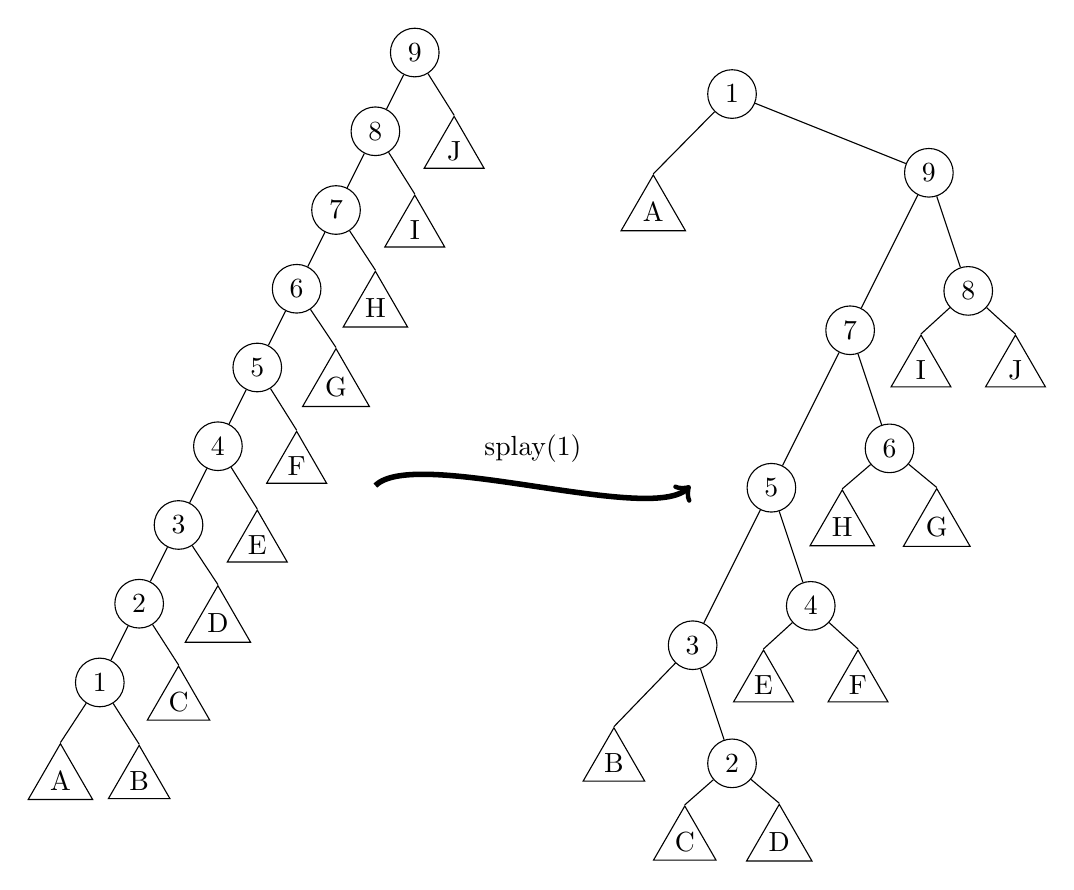
\begin{tikzpicture}[nodes=draw,shape=circle,scale=0.5]
\tikzstyle{subtree}=[regular polygon,regular polygon sides=3,inner sep=1]
\begin{scope}
\foreach \x in {1,2,...,9}{
\node(\x) at (\x, 2*\x) {\x};
};
\foreach \x/\y in {1/B,2/C,3/D,4/E,5/F,6/G,7/H,8/I,9/J}{
\node[subtree] (\y) at (\x+1, 2*\x-2.5) {\y};
\draw (\x) -- (\y.north);
};
\foreach \x/\y in {1/2,2/3,3/4,4/5,5/6,6/7,7/8,8/9}{
\draw (\x) -- (\y);
}
\node[subtree] (A) at (0,-0.5) {A};
\draw (A.north) -- (1);
\end{scope}
\draw[->,line width=2] (8,7) .. controls (9,8) and (15,6) .. (16,7) node[below=-1.3,midway,draw=none] {splay(1)};
\begin{scope}[xshift=400,yshift=-30]
\foreach \x/\y in {2/3,4/5,6/7,8/9}{
\node (\y) at (\x, 2*\x) {\y};
\node(\x) at (\x+1, 2*\y-5) {\x};
\draw (\x) -- (\y);
};

\foreach \x/\y in {3/5,5/7,7/9}{
\draw (\x) -- (\y);
}
\foreach \x/\y in {2/C,4/E,6/H,8/I}{
\node[subtree] (\y) at (\x-0.2,2*\x-5) {\y};
\draw (\x) -- (\y.north);
}

\foreach \x/\y in {2/D,4/F,6/G,8/J}{
\node[subtree] (\y) at (\x+2.2,2*\x-5) {\y};
\draw (\x) -- (\y.north);
}
\node (1) at(3, 18) {1};
\draw (1) -- (9);
\node[subtree] (A) at (1, 15) {A};
\node[subtree](B) at (0,1) {B};
\draw(1) -- (A.north);
\draw(3) -- (B.north);
\end{scope}
\end{tikzpicture}

\end{center}
\caption{\label{ziggo}Result of a splay operation on the leaf of linear height tree. The height of the tree is roughly two times smaller after the operation.}
\end{figure}
\subsection{Analysis}
To analyze a amortized complexity of a splay operation we will use the potential method. Lets consider an arbitrary function $w$ mapping nodes of a tree to positive real numbers. We will define potential function in terms of weight function $w$, prove a bound for amortized complexity of a splay operation in terms of $w$. Then, taking different functions as $w$ various properties (as static optimality, or working set property) will follow.

Indeed, for a weight function $w$, and a node $x$ of a tree let us define $s(x) := \sum_{y \in \mathrm{subtree}(x)} w(y)$ then $r(x) := \log(s(x))$ and finally:
\begin{equation*}
\Phi(S) := \sum_{x \, \mathrm{node}} r(x)
\end{equation*}

Where $\Phi$ is potential function of interests. The main lemma is presented below. Note that by taking constant weight function, simple consequence of this lemma is that amortized cost of a single operation is upper bounded by $\Oh(\log n)$.
\begin{lemma}
Amortized cost of a  single splay($x$) operation is $\Oh(1 + \log\frac{W}{s(x)})$, where $W$ is sum of weights of all items.
\end{lemma}
\begin{proof}
We want to bound amortized cost of the three basic operations: zig, zig-zig, and zig-zag. Let us say, that $r'(x)$ is defined as $r$ on node $x$ after performing an operation, and $r(x)$ would be the value before performing an operation. If we had that amortized cost of zig-zig, and zig-zag on node $x$ were at most $3(r'(x) - r(x))$, and amortized cost of zig were at most $3 (r'(x) - r(x)) + 3$, then by summing over all basic operations in a splay operation, and telescoping the sum of we would obtain that cost of a splay operation is bounded by $3 + r'(\mathrm{root}) - r(x) = \Oh(1 + \log(\frac{W}{r(x)}))$.

Thus all we have to prove is that the amortized cost of each operation is as claimed. We will prove it only for zig-zag case, as it is the most interesting --- the remaining cases are similar.

We want to show that amortized cost of zig-zig operation is not greater than $3(r'(x) - r(x))$. As the amortized cost is by definition equal to the real cost plus difference in potential, whereas the real cost is equal to $2$, what we really need is to upper bound the difference in potential by $3(r'(x) - r(x)) - 2$. Once again, let $y$ be a parent of $x$, and $z$ be a parent of $y$ as on Figure~\ref{zig-zig}. Now it is easy to see, that $r(p) = r'(p)$ when $p \not\in \{x,y,z\}$. Therefore the difference in potential is equal:
\begin{align*}
\Delta\Phi & = r'(x) + r'(y) + r'(z) - r(x) - r(y) - r(z) \\
	& = r'(y) + r'(z) - r(x) - r(y) \\
	& \leq r'(y) + r'(z) - 2r(x) \\
	& \leq r'(x) + r'(z) - 2r(x)
\end{align*}

Where the first equality is justified by $r'(x) = r(z)$, and two last inequalities are just of form $r(y) \geq r(x)$ and $r'(y) \leq r'(x)$. Now we want to bound $r'(z)$:

\begin{align*}
\frac{r(x) + r'(z)}{2} &= \log(\sqrt{s(x)s'(z)}) \\
	& \leq \log(\frac{s(x) + s'(z)}{2}) \\
	& \leq \log(\frac{s'(x)}{2}) \\
	& = r'(x) - 1
\end{align*}

Where $s(x) + s'(z) \leq s'(x)$ follows from the fact, that subtree rooted at $x$ in tree before the operation is completely disjoint (in terms of node set) with the subtree rooted at $z$ after the operation. Moreover, both those subtrees are contained in the subtree rooted in $x$ of a tree after the operation.

Rearranging terms we have:
\begin{equation*}
	r'(z) \leq 2r'(x) - r(x) - 2
\end{equation*}

Now we plug this into the bound for a difference of potential:
\begin{align*}
\Delta\Phi & \leq r'(x) + r'(z) - 2r(x) \\
	& \leq 3 (r'(x) - r(x)) - 2
\end{align*}

We obtained desired bound on the difference of potential in single zig-zig step. The amortized cost of this step is hence upper bounded by $3(r'(x) - r(x))$. One can obtain a same bound for a zig-zag step, and a similar (up to constant) for a zig step. In every splay operation, a zig step is performed at most once, the total cost of the splay operation is upper bounded by a sum of expressions of form $3(r'(x) - r(x)$, and this sum telescopes to a $\Oh(1 + r'(\mathrm{root}) - r(x))$, which is $\Oh(1 + \log\frac{W}{s(x)})$.
\end{proof}
\section{Concrete amortized complexity bounds}
As noted before stating the main lemma, by setting a constant weight function $w \equiv 1$, we get a $\Oh(\log n)$ upper bound on amortized complexity of single operation --- thus splay trees are, in average, at least as good as balanced BSTs. We will see how to set a weight function to prove a slightly weaker version of static optimality. The argument below is due to a LiveJournal post of David Eppstein, whose goal was to present static optimality of splay trees in a way that avoids mention of Shannon entropy as was done in the original paper \cite{DBLP:journals/jacm/SleatorT85}.

Consider a tree $T$, and let $l_i$ be the level on which element $i$ is in tree $T$, and let $m_i$ to be the number of times that $i$ were accessed in the access sequence under consideration.
Note that cost of processing this sequence with a tree $T$ is $\Oh(m + \sum_{i=1}^n m_i l_i)$. We will prove that for splay trees this cost is at most $\Oh(m + n^2 + \sum_{i=1}^n m_i l_i)$. Lets take the weight function $w(i) = 3^{-l_i}$. Note that with non integral weights potential function might take negative values --- this is not a problem, we still have the important property:
\begin{equation*}
\mathrm{amortized\_time} = \mathrm{actual\_time} + \Delta\Phi
\end{equation*}
hence
\begin{equation*}
\mathrm{actual\_time} = \mathrm{amortized\_time} - \Delta\Phi
\end{equation*}

First note that sum of all weights of a tree is at most constant:
\begin{equation*}
	W = \sum_{i} w_i = \sum_{l} \frac{1}{3^l} (\# \text{nodes at height }l) \leq \sum_l \left( \frac{2}{3} \right)^l \leq C
\end{equation*}

We observe that $\Phi$ takes values in the interval $[-c n^2, C' n]$ --- indeed: $w(i) \geq 3^{-n}$, so  $s(x) \geq 3^{-n}$, then $r(x) \geq -c n$, and $\sum_x r(x) \geq -c n^2$. On the other hand sum of all weights is at most constant, so $s(x) \leq C$, and $r(x) \leq C'$ --- sum of all $r(x)$ is at most $C' n$.  Now, as $\Phi$ takes values in an interval of length $\Oh(n^2)$, we conclude that $- \Delta\Phi = \Oh(n^2)$.

We need to prove that amortized time is at most $\Oh(m + \sum_{i=1}^n m^i l_i)$. By the main lemma, amortized cost of a single operation is at most $\Oh(1 + \log(\frac{W}{s(i)}))$, and as $W$ is constant, and $s(i) \geq 3^{-l_i}$ this cost is upper bounded by $\Oh(1 + \log(3^{l_i})) = \Oh(l_i)$, and amortized cost of a whole sequence is indeed $\sum_{i=1}^n l_i m_i$.
\qed

\bibliography{lec7}{}
\bibliographystyle{plain}
\end{document}
